\documentclass[11pt,a4paper]{article}
\usepackage[utf8]{inputenc}
\usepackage[margin=0.8in]{geometry}
\usepackage{tikz}
\usetikzlibrary{shapes.geometric, arrows, positioning, calc, fit, backgrounds}
\usepackage{xcolor}
\usepackage{hyperref}
\usepackage{listings}
\usepackage{enumitem}
\usepackage{tcolorbox}

% Define colors
\definecolor{startcolor}{RGB}{76, 175, 80}
\definecolor{endcolor}{RGB}{244, 67, 54}
\definecolor{processcolor}{RGB}{33, 150, 243}
\definecolor{decisioncolor}{RGB}{255, 193, 7}
\definecolor{actioncolor}{RGB}{156, 39, 176}
\definecolor{issuecolor}{RGB}{255, 87, 34}
\definecolor{fixedcolor}{RGB}{76, 175, 80}
\definecolor{warningcolor}{RGB}{255, 152, 0}

% TikZ styles - IMPROVED to match flowchart document
\tikzstyle{startstop} = [rectangle, rounded corners, minimum width=3cm, minimum height=1cm, text centered, draw=black, fill=startcolor!30, align=center]
\tikzstyle{process} = [rectangle, minimum width=3cm, minimum height=1cm, text centered, draw=black, fill=processcolor!30, align=center]
\tikzstyle{decision} = [diamond, minimum width=3.5cm, minimum height=1.2cm, text centered, draw=black, fill=decisioncolor!30, aspect=3, align=center, text width=2.5cm]
\tikzstyle{action} = [rectangle, rounded corners, minimum width=3cm, minimum height=1cm, text centered, draw=black, fill=actioncolor!30, align=center]
\tikzstyle{arrow} = [thick,->,>=stealth, rounded corners]
\tikzstyle{state} = [rectangle, rounded corners, minimum width=3cm, minimum height=1cm, text centered, draw=black, fill=blue!20, align=center, text width=3cm]

\title{\textbf{DecodeShootingAuto v5.1}\\Complete System Documentation\\January 27, 2026 Updates}
\author{FTC Robot Autonomous System}
\date{January 27, 2026}

\begin{document}

\maketitle
\tableofcontents
\newpage

% ============================================================================
\section{Update Summary - January 25-27, 2026}
% ============================================================================

\subsection{Major Changes This Session}

\begin{enumerate}
    \item \textbf{Fixed Shooter Power Control Method} - Identified velocity PID conflict
    \item \textbf{Added AprilTag Detection Debugging} - Camera streaming wait and telemetry
    \item \textbf{Created A3 OpMode} - Smart auto-indexing TeleOp with manual override
    \item \textbf{Fixed Kicker Servo Positions} - Matched SimpleRevolver working values
    \item \textbf{Fixed Kicker FSM Conflict} - Added flag to disable FSM kicker control
    \item \textbf{Implemented Timer-Based Kicking} - Direct control in A3 bypassing FSM
\end{enumerate}

\subsection{Current Issues}

\begin{tcolorbox}[colback=warningcolor!10, colframe=warningcolor, title=Open Investigation]
\textbf{Shooter Power Not Matching Commanded Value}\\
Despite setting \texttt{SHOOTER\_POWER = 0.4}, the shooter appears to run at a higher speed.\\
\textbf{Root Cause Under Investigation:}
\begin{itemize}
    \item \texttt{setShooterPower()} calls both \texttt{setVelocity()} AND \texttt{setPower()}
    \item Velocity PID may override raw power setting
    \item Currently using \texttt{setShooterPowerDirect()} to bypass velocity control
    \item \textbf{More testing needed} to confirm actual motor behavior
\end{itemize}
\end{tcolorbox}

\newpage
% ============================================================================
\section{Shooter Power Control Analysis}
% ============================================================================

\subsection{The Problem}

User observed that despite setting \texttt{SHOOTER\_POWER = 0.4}, the shooter motor appeared to run at maximum speed.

\subsection{Method Comparison}

\begin{center}
\begin{tabular}{|l|l|l|}
\hline
\textbf{Method} & \textbf{Implementation} & \textbf{Effect} \\
\hline
\texttt{setShooterPower(power)} & \begin{tabular}[c]{@{}l@{}}\texttt{setVelocity(power * 3000)}\\\texttt{setPower(power)}\end{tabular} & Velocity PID active \\
\hline
\texttt{setShooterPowerDirect(power)} & \texttt{setPower(power)} & Raw PWM only \\
\hline
\end{tabular}
\end{center}

\subsection{Analysis}

\begin{tcolorbox}[colback=issuecolor!10, colframe=issuecolor, title=Velocity PID Conflict]
When \texttt{setShooterPower(0.4)} is called:
\begin{enumerate}
    \item \texttt{setVelocity(1200)} tells motor to maintain 1200 ticks/sec
    \item \texttt{setPower(0.4)} is ignored because velocity mode is active
    \item Motor PID drives hard to reach target velocity $\rightarrow$ appears at max power
\end{enumerate}
\end{tcolorbox}

\subsection{Current Status}

\begin{itemize}
    \item Autonomous uses \texttt{setShooterPowerDirect(SHOOTER\_POWER)}
    \item Manual mode (A1) uses \texttt{setShooterPower(0.67)}
    \item \textbf{Needs Further Investigation:} Actual motor velocity vs commanded power
\end{itemize}

\newpage
% ============================================================================
\section{A3 OpMode - Smart Auto-Indexing}
% ============================================================================

\subsection{Overview}

New TeleOp mode combining A1's manual controls with autonomous-style smart indexing.

\subsection{Key Features}

\begin{itemize}
    \item \textbf{Auto-Indexing:} Detects balls during intake, rotates indexer automatically
    \item \textbf{Manual Override:} Cross button and D-pad still work
    \item \textbf{Direct Kicker Control:} Bypasses RevolverSubsystem FSM
    \item \textbf{Edge Detection:} Prevents double-triggering with 800ms cooldown
\end{itemize}

\subsection{Control Mapping}

\begin{center}
\begin{tabular}{|l|l|}
\hline
\textbf{Button} & \textbf{Function} \\
\hline
RT & Intake + Auto-index \\
LT & Reverse intake \\
Circle & Toggle shooter \\
LB & Kick (timer-based) \\
Cross & Manual index \\
D-pad Up/Down & Manual trim $\pm$5 ticks \\
RB & Slow drive mode \\
\hline
\end{tabular}
\end{center}

\subsection{Auto-Indexing Flow}

\begin{center}
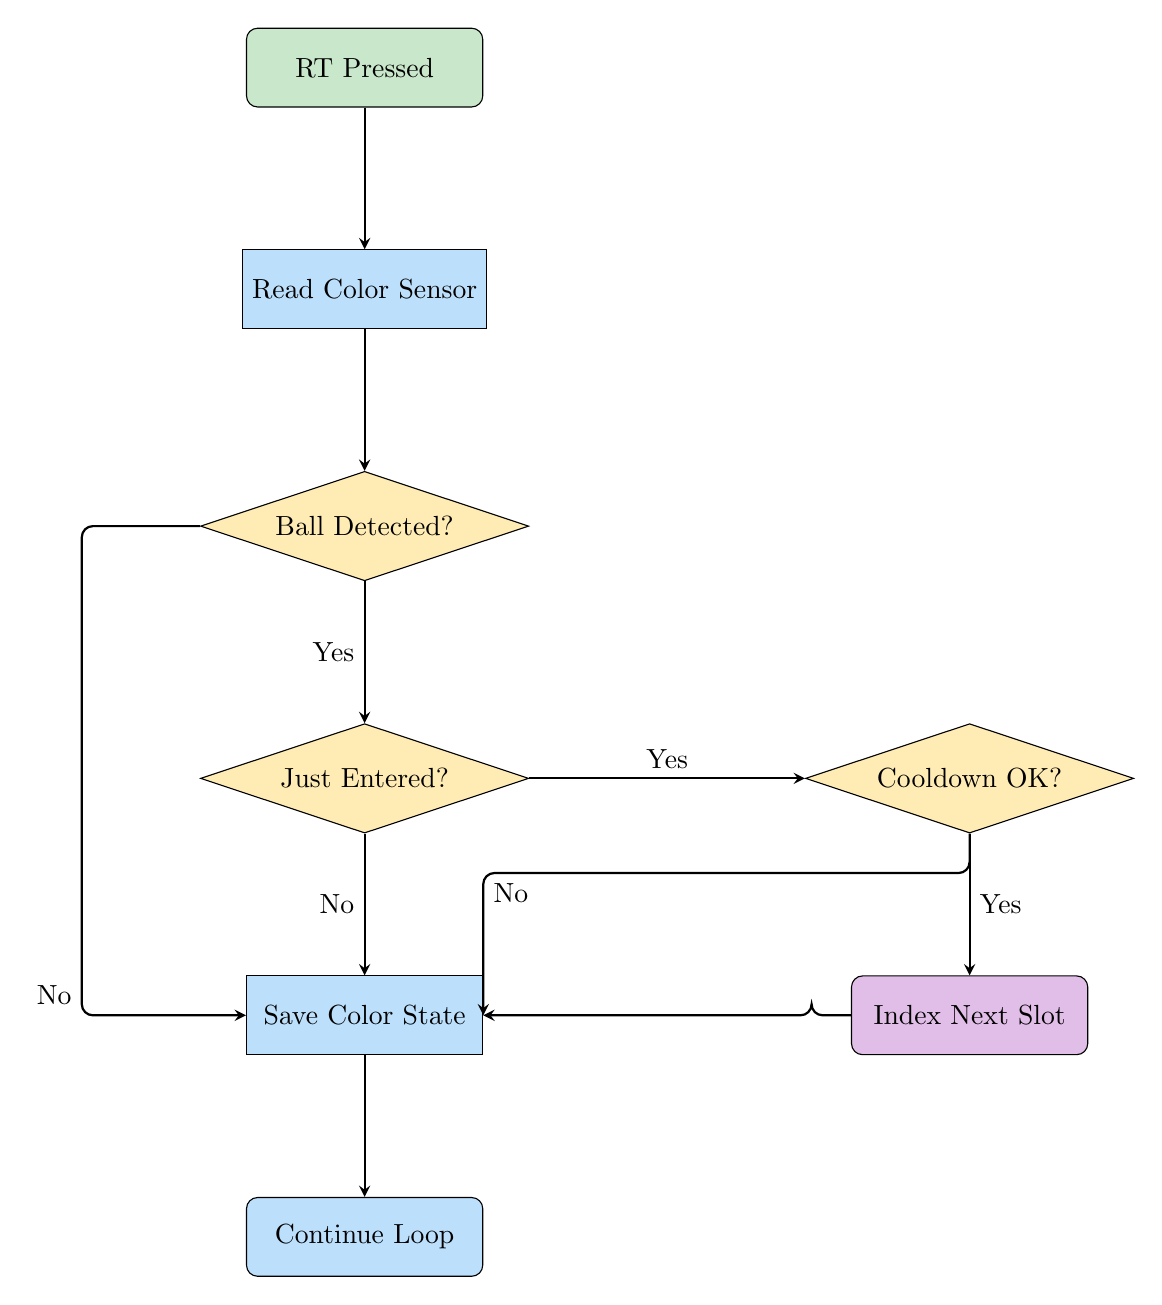
\begin{tikzpicture}[node distance=1.8cm, auto]

% Main vertical spine
\node (rt) [startstop] {RT Pressed};
\node (read) [process, below=of rt] {Read Color Sensor};
\node (detect) [decision, below=of read] {Ball Detected?};
\node (edge) [decision, below=of detect] {Just Entered?};
\node (save) [process, below=of edge] {Save Color State};
\node (cont) [startstop, below=of save, fill=processcolor!30] {Continue Loop};

% Right branch for successful detection
\node (cool) [decision, right=3.5cm of edge] {Cooldown OK?};
\node (index) [action, below=of cool] {Index Next Slot};

% Arrows - main spine
\draw [arrow] (rt) -- (read);
\draw [arrow] (read) -- (detect);
\draw [arrow] (detect) -- node[left] {Yes} (edge);
\draw [arrow] (edge) -- node[left] {No} (save);
\draw [arrow] (save) -- (cont);

% No detection path - route around edge node
\draw [arrow] (detect.west) -- ++(-1.5,0) |- node[above left] {No} (save.west);

% Edge detection to cooldown
\draw [arrow] (edge) -- node[above] {Yes} (cool);

% Cooldown paths
\draw [arrow] (cool) -- node[right] {Yes} (index);
\draw [arrow] (index.west) -- ++(-0.5,0) |- (save.east);

% Cooldown No path
\draw [arrow] (cool.south) -- ++(0,-0.5) -| node[below right] {No} (save.east);

\end{tikzpicture}
\end{center}

\newpage
% ============================================================================
\section{Kicker Control - Fixes Applied}
% ============================================================================

\subsection{Problems Encountered}

\begin{enumerate}
    \item \textbf{Kicker Retracting Immediately:} FSM LOADING state constantly set kicker to retract
    \item \textbf{Wrong Servo Positions:} RevolverSubsystem used different values than SimpleRevolver
    \item \textbf{No Timer Sequence:} Direct \texttt{kickerEject()} had no timing control
\end{enumerate}

\subsection{Servo Position Correction}

\begin{center}
\begin{tabular}{|l|c|c|c|}
\hline
\textbf{Position} & \textbf{SimpleRevolver (A1)} & \textbf{Old RevolverSubsystem} & \textbf{Fixed Value} \\
\hline
RETRACT & 0.3 & 0.5 & \textbf{0.3} \\
EJECT & 0.8 & 1.0 & \textbf{0.8} \\
\hline
\end{tabular}
\end{center}

\subsection{Timer-Based Kick Sequence}

Both SimpleRevolver (A1) and now A3 use this sequence:

\begin{center}
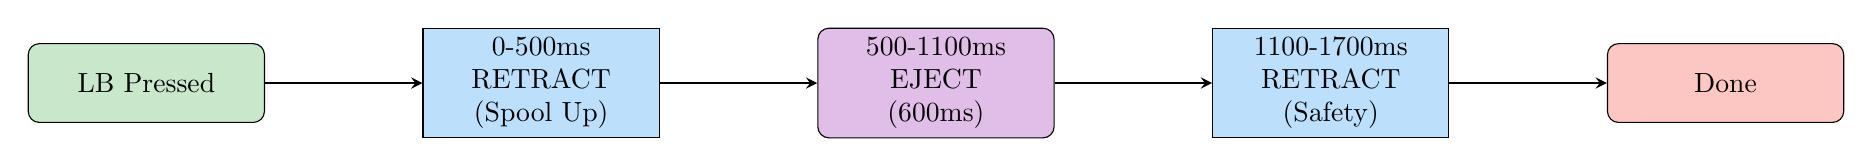
\begin{tikzpicture}[node distance=2cm, auto]

% Horizontal flow
\node (start) [startstop] {LB Pressed};
\node (spool) [process, right=of start, text width=2.5cm] {0-500ms\\RETRACT\\(Spool Up)};
\node (eject) [action, right=of spool, text width=2.5cm] {500-1100ms\\EJECT\\(600ms)};
\node (retract) [process, right=of eject, text width=2.5cm] {1100-1700ms\\RETRACT\\(Safety)};
\node (done) [startstop, right=of retract, fill=endcolor!30] {Done};

% Simple straight arrows
\draw [arrow] (start) -- (spool);
\draw [arrow] (spool) -- (eject);
\draw [arrow] (eject) -- (retract);
\draw [arrow] (retract) -- (done);

\end{tikzpicture}
\end{center}

\subsection{FSM Conflict Resolution}

\begin{tcolorbox}[colback=fixedcolor!10, colframe=fixedcolor, title=Solution: Direct Control Flag]
Added \texttt{disableFSMKickerControl} flag to RevolverSubsystem:
\begin{verbatim}
// In A3.init():
revolver.disableFSMKickerControl = true;

// In RevolverSubsystem.update() LOADING state:
if (!disableFSMKickerControl) {
    kicker.setPosition(KICKER_RETRACT_POS);
}
\end{verbatim}
A3 directly controls kicker via \texttt{revolver.kicker.setPosition()}.
\end{tcolorbox}

\newpage
% ============================================================================
\section{AprilTag Detection Updates}
% ============================================================================

\subsection{Problem}

AprilTag detection worked during init (camera preview showed tags) but failed during autonomous execution.

\subsection{Fixes Applied}

\begin{enumerate}
    \item \textbf{Camera Streaming Wait:} Added wait loop during init to ensure VisionPortal is streaming
    \item \textbf{Enhanced Telemetry:} Shows detection count and camera state during detection phase
    \item \textbf{Made Vision Components Public:} \texttt{aprilTag} and \texttt{visionPortal} for telemetry access
\end{enumerate}

\subsection{Init Phase Monitoring}

\begin{verbatim}
// CRITICAL: Wait for camera to start streaming
while (!isStarted() && !isStopRequested()) {
    telemetry.addData("Camera Status", 
        tagNavigator.visionPortal.getCameraState());
    telemetry.addData("Detections", 
        tagNavigator.aprilTag.getDetections().size());
    telemetry.update();
    sleep(20);
}
\end{verbatim}

\subsection{Current Status}

\begin{tcolorbox}[colback=warningcolor!10, colframe=warningcolor, title=Needs Testing]
Camera streaming wait added. User should verify:
\begin{itemize}
    \item Camera shows \texttt{STREAMING} status during init
    \item Detections count > 0 when tags visible
    \item Tags detected during autonomous execution
\end{itemize}
\end{tcolorbox}

\newpage
% ============================================================================
\section{RevolverSubsystem State Machine}
% ============================================================================

\subsection{State Diagram}

\begin{center}
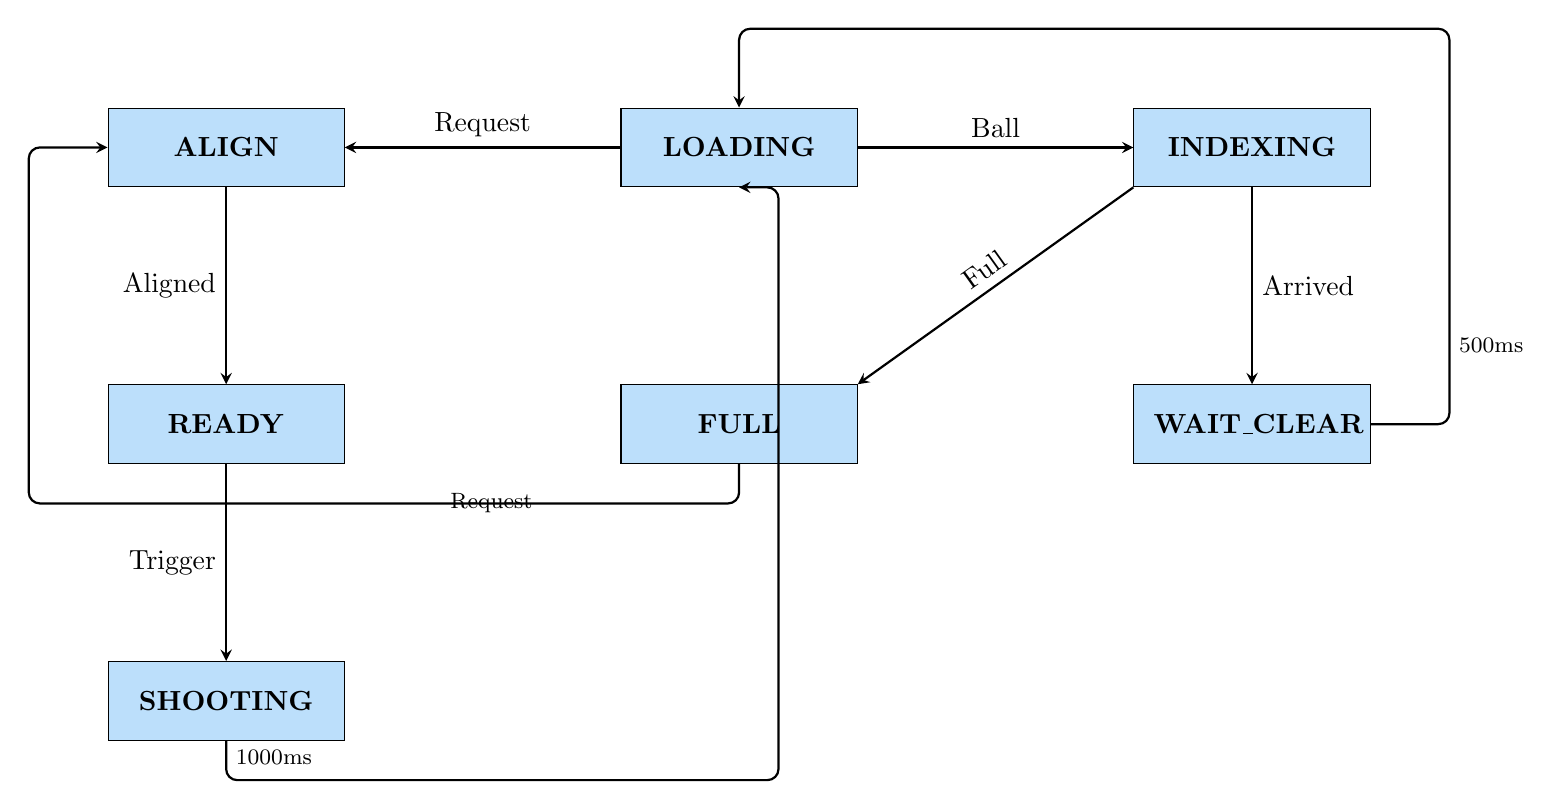
\begin{tikzpicture}[node distance=2.5cm, auto]

% Setup with wide spacing to avoid crossings
\node (loading) [process, text width=2.5cm] {\textbf{LOADING}};

% Right Column (Intake path)
\node (indexing) [process, right=3.5cm of loading, text width=2.5cm] {\textbf{INDEXING}};
\node (wait) [process, below=of indexing, text width=2.5cm] {\textbf{WAIT\_CLEAR}};

% Center Bottom
\node (full) [process, below=of loading, text width=2.5cm] {\textbf{FULL}};

% Left Column (Shooting path)
\node (align) [process, left=3.5cm of loading, text width=2.5cm] {\textbf{ALIGN}};
\node (ready) [process, below=of align, text width=2.5cm] {\textbf{READY}};
\node (shooting) [process, below=of ready, text width=2.5cm] {\textbf{SHOOTING}};

% --- Transitions with Explicit Routing ---

% 1. Loading -> Indexing (Straight)
\draw [arrow] (loading) -- node[above] {Ball} (indexing);

% 2. Indexing -> Wait (Straight Down)
\draw [arrow] (indexing) -- node[right] {Arrived} (wait);

% 3. Wait -> Loading (Wide path above everything)
\draw [arrow] (wait.east) -- ++(1,0) |- ([yshift=1cm]loading.north) -- (loading.north);
\node [right, font=\footnotesize] at ($(wait.east)+(1,1)$) {500ms};

% 4. Indexing -> Full (Diagonal path)
\draw [arrow] (indexing.south west) -- node[sloped, above] {Full} (full.north east);

% 5. Loading -> Align (Straight)
\draw [arrow] (loading) -- node[above] {Request} (align);

% 6. Full -> Align (Wide path below and left)
\draw [arrow] (full.south) -- ++(0,-0.5) -| ([xshift=-1cm]align.west) -- (align.west);
\node [left, font=\footnotesize] at ($(full.south)+(-2.5,-0.5)$) {Request};

% 7. Align -> Ready (Straight Down)
\draw [arrow] (align) -- node[left] {Aligned} (ready);

% 8. Ready -> Shooting (Straight Down)
\draw [arrow] (ready) -- node[left] {Trigger} (shooting);

% 9. Shooting -> Loading (Wide path below and right)
\draw [arrow] (shooting.south) -- ++(0,-0.5) -| ([xshift=0.5cm]loading.south) -- (loading.south);
\node [below right, font=\footnotesize] at (shooting.south) {1000ms};

\end{tikzpicture}
\end{center}

\subsection{State Descriptions}

\begin{description}
    \item[LOADING] Empty slot at intake position (0°), waiting for ball
    \item[INDEXING] Moving indexer to next empty slot
    \item[WAIT\_FOR\_INTAKE\_CLEAR] Pause after indexing (500ms)
    \item[FULL] All 3 slots filled
    \item[SHOOTING\_ALIGN] Rotating target slot to shooter position (240°)
    \item[READY\_TO\_SHOOT] Aligned, waiting for manual trigger
    \item[SHOOTING] Kicker sequence active (1000ms)
\end{description}

\newpage
% ============================================================================
\section{Color Sensor Detection Logic}
% ============================================================================

\subsection{Detection Flow}

\begin{center}
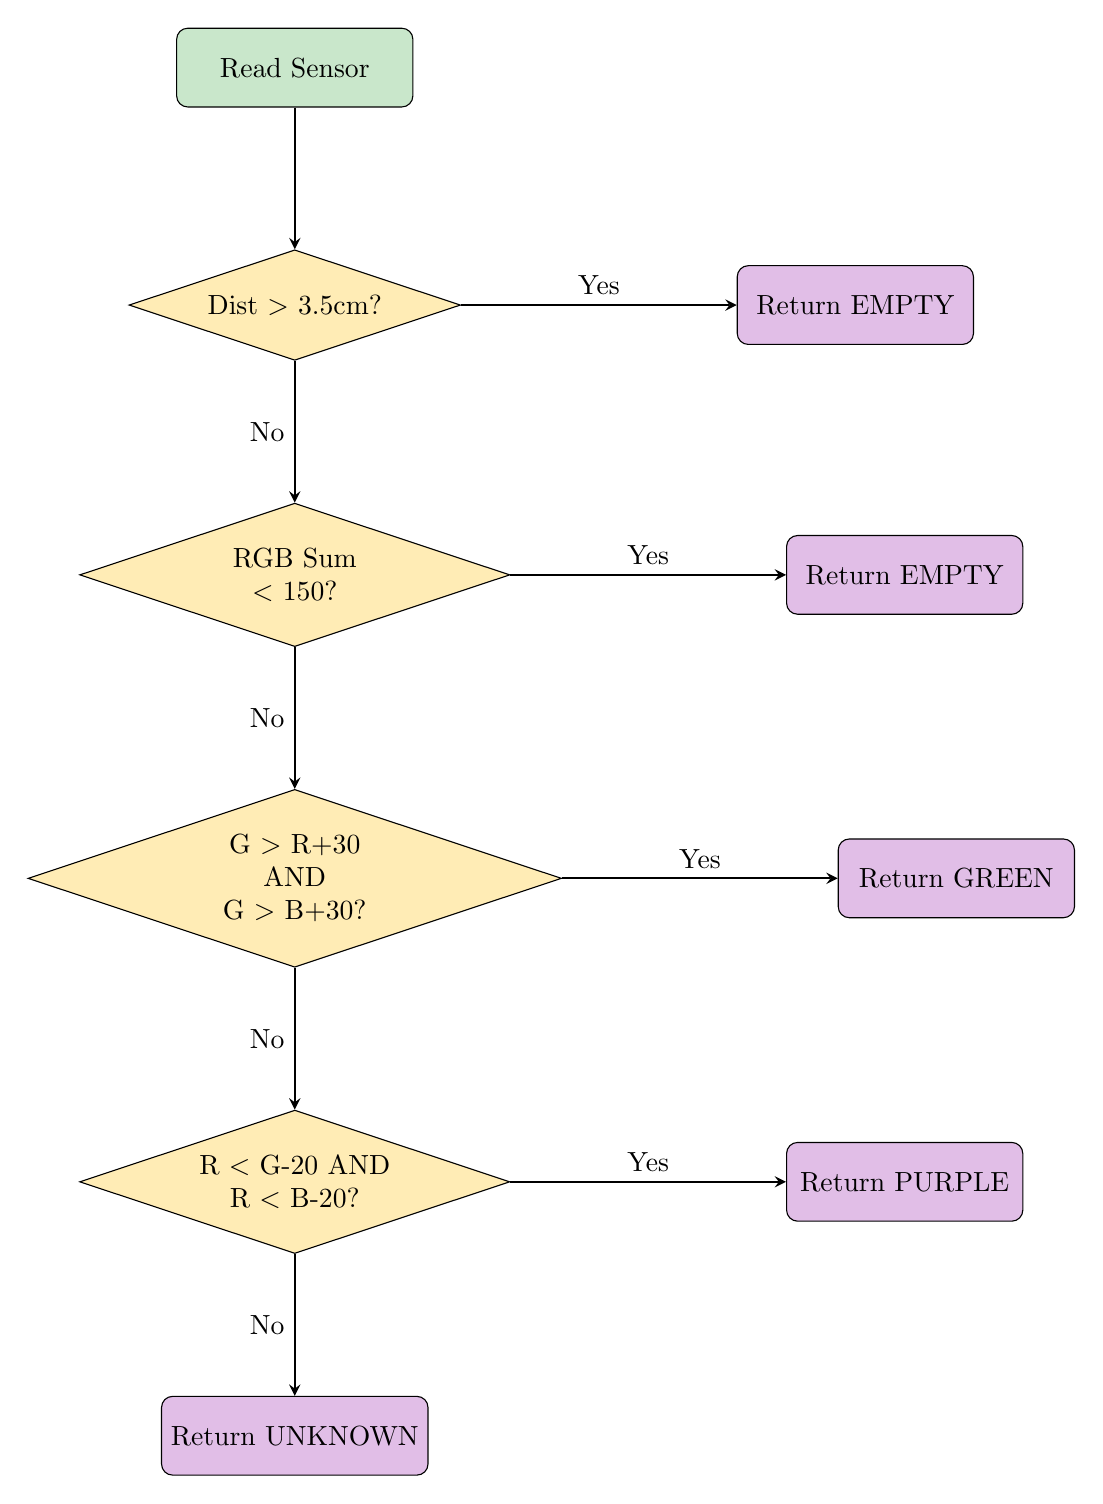
\begin{tikzpicture}[node distance=1.8cm, auto]

% Main Vertical Spine
\node (start) [startstop] {Read Sensor};
\node (dist) [decision, below=of start] {Dist $>$ 3.5cm?};
\node (bright) [decision, below=of dist] {RGB Sum $<$ 150?};
\node (green) [decision, below=of bright] {G $>$ R+30 AND\\G $>$ B+30?};
\node (purple) [decision, below=of green] {R $<$ G-20 AND\\R $<$ B-20?};
\node (unknown) [action, below=of purple] {Return UNKNOWN};

% Results (Right side) - positioned to avoid crossings
\node (empty1) [action, right=3.5cm of dist] {Return EMPTY};
\node (empty2) [action, right=3.5cm of bright] {Return EMPTY};
\node (gret) [action, right=3.5cm of green] {Return GREEN};
\node (pret) [action, right=3.5cm of purple] {Return PURPLE};

% Arrows - Main spine
\draw [arrow] (start) -- (dist);

% Distance Check
\draw [arrow] (dist) -- node[above] {Yes} (empty1);
\draw [arrow] (dist) -- node[left] {No} (bright);

% Brightness Check
\draw [arrow] (bright) -- node[above] {Yes} (empty2);
\draw [arrow] (bright) -- node[left] {No} (green);

% Green Check
\draw [arrow] (green) -- node[above] {Yes} (gret);
\draw [arrow] (green) -- node[left] {No} (purple);

% Purple Check
\draw [arrow] (purple) -- node[above] {Yes} (pret);
\draw [arrow] (purple) -- node[left] {No} (unknown);

\end{tikzpicture}
\end{center}

\subsection{Detection Thresholds}

\begin{center}
\begin{tabular}{|l|c|l|}
\hline
\textbf{Parameter} & \textbf{Value} & \textbf{Purpose} \\
\hline
COLOR\_DETECT\_DISTANCE\_CM & 3.5 & Max distance to detect ball \\
Minimum Brightness (R+G+B) & 150 & Avoid scattered light \\
\hline
\multicolumn{3}{|c|}{\textbf{GREEN Detection}} \\
\hline
Condition & \texttt{G > R+30 AND G > B+30} & Green dominates both \\
\hline
\multicolumn{3}{|c|}{\textbf{PURPLE Detection}} \\
\hline
Condition & \texttt{R < G-20 AND R < B-20} & Red is lowest \\
\hline
\end{tabular}
\end{center}

\newpage
% ============================================================================
\section{Complete Autonomous Flow}
% ============================================================================

\begin{center}
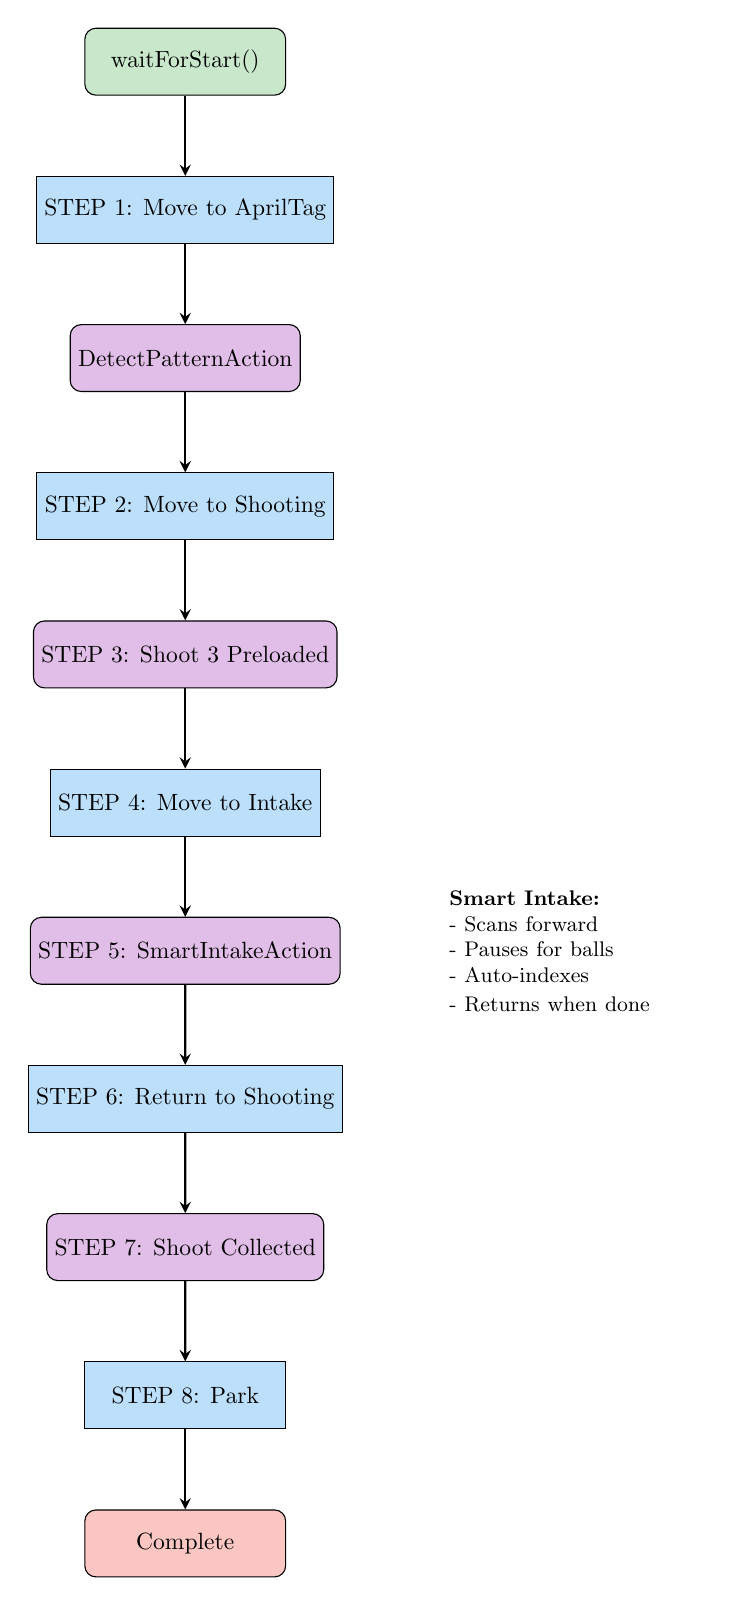
\begin{tikzpicture}[node distance=1.2cm, scale=0.85, transform shape]

% Nodes - vertical flow
\node (start) [startstop] {waitForStart()};
\node (step1) [process, below=of start] {STEP 1: Move to AprilTag};
\node (detect) [action, below=of step1] {DetectPatternAction};
\node (step2) [process, below=of detect] {STEP 2: Move to Shooting};
\node (step3) [action, below=of step2] {STEP 3: Shoot 3 Preloaded};
\node (step4) [process, below=of step3] {STEP 4: Move to Intake};
\node (step5) [action, below=of step4] {STEP 5: SmartIntakeAction};
\node (step6) [process, below=of step5] {STEP 6: Return to Shooting};
\node (step7) [action, below=of step6] {STEP 7: Shoot Collected};
\node (step8) [process, below=of step7] {STEP 8: Park};
\node (end) [startstop, below=of step8, fill=endcolor!30] {Complete};

% Simple straight arrows
\draw [arrow] (start) -- (step1);
\draw [arrow] (step1) -- (detect);
\draw [arrow] (detect) -- (step2);
\draw [arrow] (step2) -- (step3);
\draw [arrow] (step3) -- (step4);
\draw [arrow] (step4) -- (step5);
\draw [arrow] (step5) -- (step6);
\draw [arrow] (step6) -- (step7);
\draw [arrow] (step7) -- (step8);
\draw [arrow] (step8) -- (end);

% Annotations on right side
\node[right=1.5cm of step5, text width=4cm, align=left] {
    \small
    \textbf{Smart Intake:}\\
    - Scans forward\\
    - Pauses for balls\\
    - Auto-indexes\\
    - Returns when done
};

\end{tikzpicture}
\end{center}

\newpage
% ============================================================================
\section{System Parameters Reference (Updated)}
% ============================================================================

\begin{center}
\begin{tabular}{|l|c|l|}
\hline
\textbf{Parameter} & \textbf{Value} & \textbf{Description} \\
\hline
\multicolumn{3}{|c|}{\textbf{Timing (ms)}} \\
\hline
SHOOTER\_SPINUP\_MS & 1000 & Shooter warm-up time \\
Kick Spool Time & 500 & Wait before ejecting \\
Kick Eject Duration & 600 & Kicker extended time \\
Kick Retract Duration & 600 & Safety retraction time \\
INDEXER\_SETTLE\_MS & 500 & Indexer stabilization \\
INDEX\_COOLDOWN\_MS & 800 & Auto-index debounce (A3) \\
\hline
\multicolumn{3}{|c|}{\textbf{Servo Positions}} \\
\hline
KICKER\_RETRACT & 0.3 & Retracted position \\
KICKER\_EJECT & 0.8 & Ejection position \\
\hline
\multicolumn{3}{|c|}{\textbf{Power Levels}} \\
\hline
SHOOTER\_POWER (Auto) & 0.4 & Uses setShooterPowerDirect \\
SHOOTER\_POWER (Manual) & 0.67 & Uses setShooterPower \\
INTAKE\_POWER & 1.0 & Full intake power \\
\hline
\end{tabular}
\end{center}

\newpage
% ============================================================================
\section{Recommended Next Steps}
% ============================================================================

\subsection{Priority 1: Shooter Power Investigation}

\begin{enumerate}
    \item \textbf{Add Velocity Telemetry}
    \begin{itemize}
        \item Log \texttt{shooter.getVelocity()} during operation
        \item Compare commanded vs actual velocity
    \end{itemize}
    
    \item \textbf{Test Both Methods}
    \begin{itemize}
        \item \texttt{setShooterPowerDirect(0.4)} - raw PWM
        \item \texttt{setShooterPower(0.4)} - velocity + power
        \item Measure actual ball exit speed/distance
    \end{itemize}
    
    \item \textbf{Consider Motor Mode}
    \begin{itemize}
        \item Check if motor is in \texttt{RUN\_USING\_ENCODER} mode
        \item Try \texttt{RUN\_WITHOUT\_ENCODER} for pure power control
    \end{itemize}
\end{enumerate}

\subsection{Priority 2: AprilTag Verification}

\begin{enumerate}
    \item Verify camera shows \texttt{STREAMING} during init
    \item Confirm detection count > 0 with tags visible
    \item Test detection during autonomous movement
\end{enumerate}

\subsection{Priority 3: A3 Field Testing}

\begin{enumerate}
    \item Verify auto-indexing triggers correctly during intake
    \item Confirm kicker works smoothly without lag
    \item Test manual override controls (Cross, D-pad)
\end{enumerate}

\end{document}
